\documentclass{resume}
\usepackage{zh_CN-Adobefonts_external, tabu, multirow, linespacing_fix, cite, titlesec, graphicx, amsmath, fontawesome5, eso-pic}

% Adjust section and subsection spacing
\titlespacing*{\section}{0pt}{0.5ex plus 0.2ex minus 0.2ex}{0.5ex plus 0.2ex}
\titlespacing*{\subsection}{0pt}{0.5ex plus 0.2ex minus 0.2ex}{0.5ex plus 0.2ex}

% Set paragraph and item spacing
\setlength{\parskip}{0.5ex}
\setlength{\itemsep}{0.5ex}

% 添加证件照背景图片(已隐去路径)
\AddToShipoutPictureBG{%
  \AtPageLowerLeft{%
    \put(456,701){%
      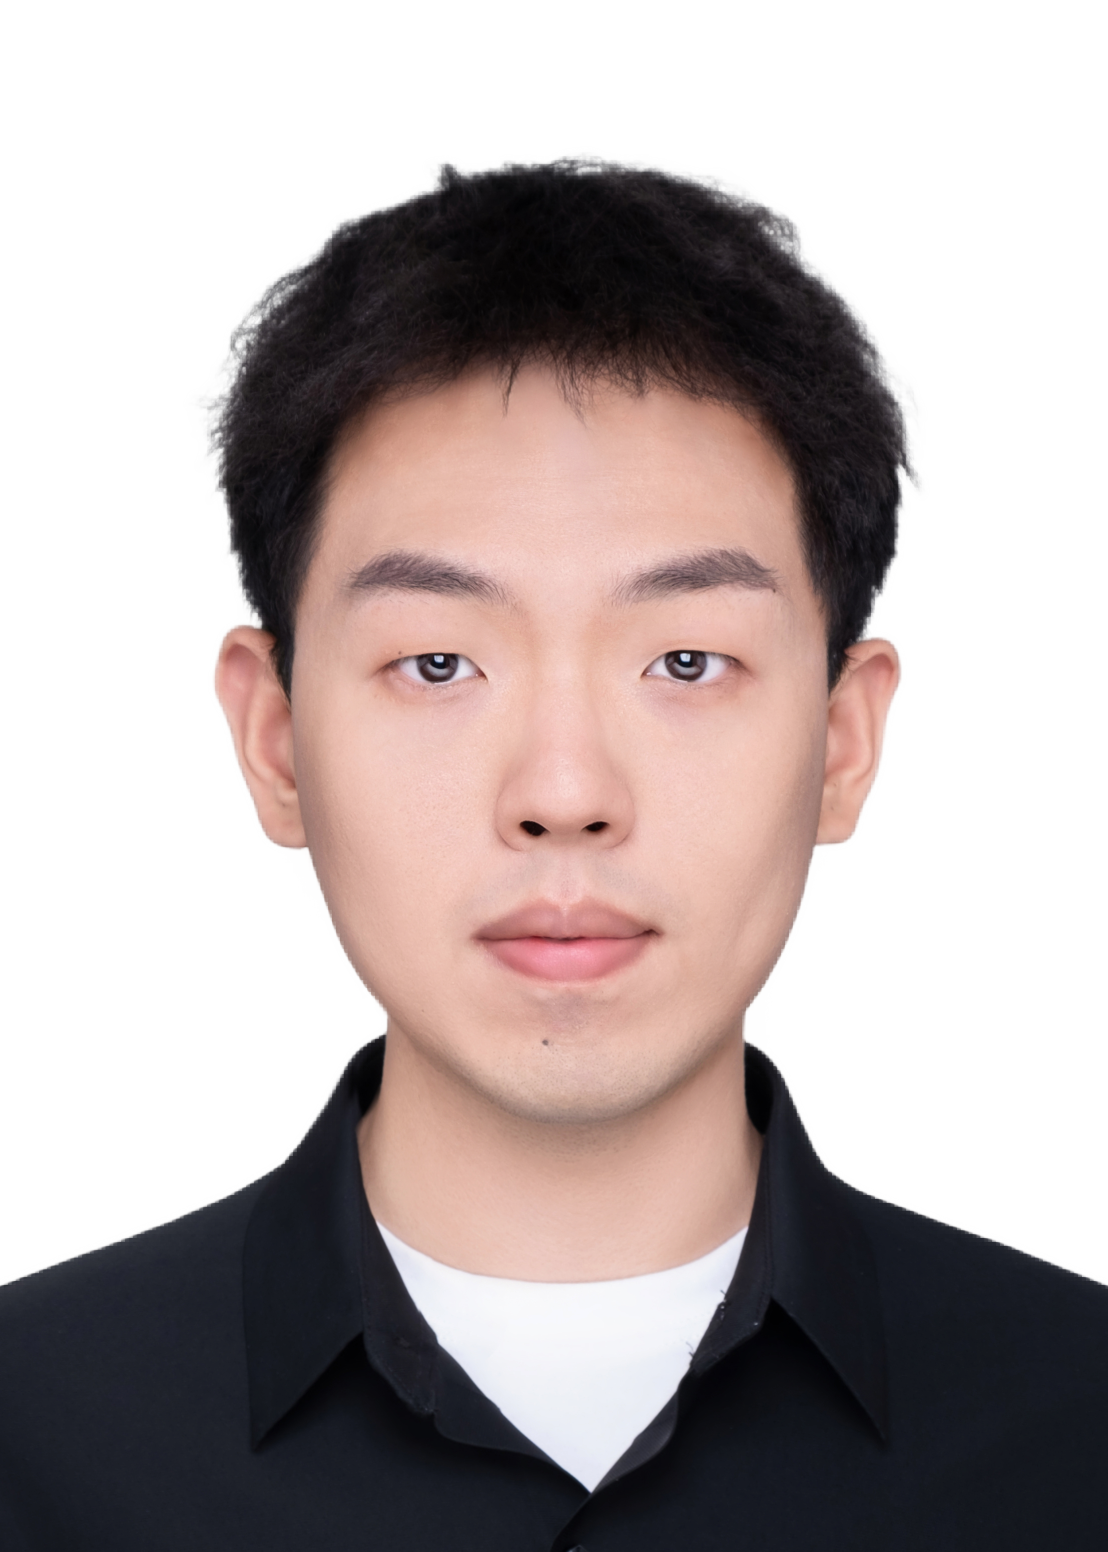
\includegraphics[width=1.15in]{avatar}
    }%
  }%
}

\begin{document}
\pagestyle{empty}
\name{[姓名]}
\basicInfo{
    \email{[邮箱]} \textperiodcentered\ 
    \phone{[手机号]} \textperiodcentered\ 
    \text{[出生年份]年[出生月份]生}
  }
\basicInfo{具备较好英语能力,计算机运维和人际沟通能力}

\section{\faGraduationCap\ 教育背景}
\datedsubsection{\textbf{国内某高校,University of XXX (XXX大学)QS162}}{[入学年份]年[入学月份] -- [毕业年份]年[毕业月份]}
\textbf{计算机技术,Computer Science(计算机科学) 双硕士学位} \\
主修科目:Python数据结构,项目管理,SQL,机器学习,密码学,数据挖掘,高阶网络安全 \\
荣获\textbf{[学年]学年全额奖学金([金额]万)},雅思考试7\textbf{(阅读8听力7)} \\
担任研究生党支部书记,主持学部日常党务工作,获国内某高校优秀研究生干部

\datedsubsection{\textbf{国内某高校}}{[入学年份]年[入学月份] -- [毕业年份]年[毕业月份]}
材料科学与工程——功能材料,工学学士(GPA[GPA数值]),英语(双学位) \\
\textbf{校级三好学生,校级二等奖学金,全国大学生英语竞赛二等奖}

\section{\faUsers\ 实习经历}
\datedsubsection{\textbf{某私募基金管理有限公司 运维工程师}}{[实习开始年份]年[实习开始月份] -- [实习结束年份]年[实习结束月份]}
\begin{itemize}
  \item 对象存储工作:针对生产环境的代码、日志、数据库等文件,利用共有云服务进行容灾;完成前期方案调研、价格调研、采购对接、部署落地、参数调优
  \item Python运维的代码优化:针对某py程序Crash后需要重新运行某一部分函数;利用Python的argparse模块以命令行的方式重新运行某段代码
  \item 服务器扩容工作:针对MongoDB数据库的慢查询问题进行排障,结论为缓存命中率低,进行Linux服务器内存扩容;针对Mysql数据库主从同步的固态硬盘空间需求,对Windows服务器进行RAID 5扩容
  \item 数据商数据部署工作:将数据商提供Docker-Compose部署方式,编写Dockerfile、利用k8s的Deployment部署方式部署。完成三个数据商、一个日内(T+0)交易软件的测试环境部署工作
\end{itemize}

\section{\faUsers\ 项目经历}
\datedsubsection{\textbf{基于多模态和rPPG技术的驾驶疲劳监测方法}}{[项目开始年份]年[项目开始月份] -- [项目结束年份]年[项目结束月份]}
计算机视觉,深度学习,Python,两项国家自然科学基金项目立项,一项结题
\begin{itemize}
  \item 基于视觉提取rPPG生理信号,获取心率,心率变异性,呼吸等相关数据
  \item 对卷积神经网络处理的多模态特征进行特征提取和处理,通过LSTM实现时序特征共享
  \item 通过特征级融合与决策及融合对多模态特征融合提取处理
  \item 3DCNN+时序归一化+SimAM注意力机制,以减半的参数实现与PhysNet模型相近的性能
  \item 项目成果《LightweightPhys: A Lightweight and Robust Network for Remote Photoplethysmography Signal Extraction》在Journal of Advanced Digital Communications(JADC)以一作身份发表
\end{itemize}

\datedsubsection{\textbf{机场跑道块状异物清除机器人}}{[项目开始年份]年[项目开始月份] -- [项目结束年份]年[项目结束月份]}
用于机场跑道的基于路径规划算法和计算机视觉的智能清扫机器人,基于OpenCV库和树莓派搭建
\begin{itemize}
  \item 作为Leader带领团队从零完成项目构建,推进和协调工作,多次担任路演角色,临场经验丰富
  \item 取得专利“ 一种机场跑道块状异物清除装置 ”立项
  \item 作为第一年立项的项目获国内某高校挑战杯一等奖,省级挑战杯二等奖,省级互联网+二等奖
\end{itemize}

\section{\faHeartO\ 科研经历}
\datedsubsection{\textbf{Automatic Knowledge Graph Construction over Efficient Information Extraction Networks\\构建在高效信息提取网络上的自动知识图谱, IEIR [会议年份]会议 }}{[项目开始年份]年[项目开始月份] -- [项目结束年份]年[项目结束月份]}
\begin{itemize}
  \item 项目背景:为了预训练模型的训练成本,提高运行速度,在不降低命名实体识别准确率的情况下,用最低成本构建特定小样本数据集的知识图谱
  \item 解决方案:CNN+Bi-LSTM+Attention机制,实现了与RoBERTa+CRF模型几乎相同的0.8243的F1-score,但运行时间只有后者的一半
\end{itemize}

\end{document}
